% ============================================================
%  Modul 6 — Otomatisasi Proses Build dengan Makefile
% ============================================================

\chapter{Otomatisasi Proses Build dengan Makefile}
\label{chap:modul-06}

% --- 1. Tujuan dan Output Praktikum ---
\section{Tujuan dan Output Praktikum}

\subsection{Tujuan Praktikum}
Setelah menyelesaikan praktikum ini, mahasiswa diharapkan mampu:
\begin{enumerate}
    \item Memahami konsep dasar otomatisasi kompilasi (\textit{build automation}) perangkat lunak.
    \item Memahami dan menjelaskan struktur dasar berkas \texttt{Makefile} (Target, Komponen Syarat, dan Resep).
    \item Menggunakan variabel kompilator dan \textit{flags} penanda dalam \texttt{Makefile}.
    \item Menggunakan variabel otomatis (\textit{automatic variables}) seperti \texttt{\$@} dan \texttt{\$\textasciicircum} untuk efisiensi skrip \textit{build}.
\end{enumerate}

\subsection{Output Praktikum}
Pada akhir praktikum ini, mahasiswa diharapkan menghasilkan:
\begin{itemize}
    \item Berkas \texttt{Makefile} yang mampu mengompilasi program dengan satu ketikan perintah.
    \item Berkas \texttt{Makefile} multi-target (termasuk fitur \texttt{clean} untuk membersihkan proyek).
    \item Kode program multi-berkas yang sukses dikompilasi menggunakan aturan \texttt{Makefile} tingkat lanjut.
\end{itemize}

% --- 2. Dasar Teori ---
\newpage
\section{Dasar Teori}

\subsection{Otomatisasi Build dan Utilitas Make}
Dalam pengembangan perangkat lunak modern, sebuah program sering kali bersumber dari ratusan bahkan ribuan berkas (\textit{files}). Mengompilasi kode tersebut satu per satu menggunakan terminal sangatlah tidak efisien dan rawan akan \textit{human error} \cite{bryant2015computer}. Oleh karena itu, diperkenalkan konsep otomatisasi sistem reka rakit (\textit{build automation}). 

\textit{GNU Make} adalah perangkat lunak standar di sistem mirip Unix yang bertugas untuk mengendalikan proses generasi berkas \textit{executable} atau berkas luaran lainnya dari kumpulan berkas kode sumber \cite{stallman2004gnu}. Make bekerja dengan cara membaca instruksi tekstual dari sebuah berkas khusus yang dinamakan \texttt{Makefile}.

\subsection{Anatomi Dasar Makefile}
Berkas \texttt{Makefile} terdiri dari sekumpulan \textbf{Aturan} (\textit{Rules}). Setiap Aturan mendikte \textit{Make} tentang kapan dan bagaimana sebuah berkas (atau target) harus dibuat ulang. Struktur formal dari sebuah aturan adalah sebagai berikut:

\begin{verbatim}
target: prerequisites (syarat/dependensi)
    recipe (perintah terminal)
\end{verbatim}

\begin{itemize}
    \item \textbf{Target}: Biasanya berupa nama berkas yang akan dihasilkan (contoh: \texttt{program.exe} atau \texttt{main.o}). Target juga bisa berupa nama aksi semu (\textit{phony target}) seperti \texttt{clean}.
    \item \textbf{Prerequisites}: (Dependensi atau prasyarat) Berkas-berkas yang dibutuhkan sebelum target bisa dieksekusi. Jika ada satu saja *prerequisite* yang lebih baru dari *target* (telah dimodifikasi), maka \textit{Make} akan menjalankan resepnya \cite{stallman2004gnu}.
    \item \textbf{Recipe}: (Resep) Perintah-perintah baris komando/terminal spesifik (\textit{shell commands}) yang harus dijalankan. \textbf{Perhatian Penting:} Karakter pertama pada setiap baris resep WAJIB menggunakan satu karakter penjarakan \textbf{TAB}, tidak boleh menggunakan spasi biasa.
\end{itemize}

\subsection{Variabel (Makro) dalam Make}
Untuk menghindari pengetikan ulang dan mempermudah perubahan konfigurasi, Makefile mendukung variabel. Misalnya, menentukan tipe kompiler.
Contoh inisialisasi: \texttt{CC = gcc}. Cara memanggilnya adalah menggunakan perisai dolar dan kurung: \texttt{\$(CC)}.

Selain variabel kustom buatan manusia, Makefile memiliki \textbf{Variabel Otomatis} (\textit{Automatic Variables}) yang nilainya dievaluasi seketika bergantung pada konteks aturannya. Tabel \ref{tab:m06-dasar-teori} merangkum beberapa hal terpenting.

\begin{table}[h]
\caption{Konvensi Variabel Makefile}
\label{tab:m06-dasar-teori}
\centering
\begin{tabulary}{\textwidth}{|L|L|}
\hline
\textbf{Konsep} & \textbf{Penjelasan Singkat} \\ \hline
\texttt{CC}        & Nama kompilator C standar, secara default diisi \texttt{gcc}. \\ \hline
\texttt{CFLAGS}    & Bendera (\textit{flags}) tambahan yang diteruskan ke kompiler, misal: \texttt{-Wall -g}. \\ \hline
\texttt{\$@}       & Alias otomatis untuk "Nama \textbf{Target}" saat ini. \\ \hline
\texttt{\$\textasciicircum}       & Alias otomatis untuk "Semua \textbf{Prerequisites}". \\ \hline
\texttt{\$<}       & Alias otomatis untuk "\textbf{Prerequisite Pertama}" saja. \\ \hline
\end{tabulary}
\end{table}

% --- 3. Alat dan Bahan ---
\newpage
\section{Alat dan Bahan}
\label{sec:m06-alat-bahan}

\subsection{Perangkat Keras}
\begin{itemize}
    \item PC/Laptop dengan arsitektur prosesor x86\_64 atau perangkat yang mendukung Linux.
    \item Penyimpanan (\textit{storage}) lokal yang cukup.
\end{itemize}

\subsection{Perangkat Lunak}
\begin{itemize}
    \item Sistem Operasi Linux (ataupun WSL/Windows Subsystem for Linux).
    \item Perkakas paket bantu \textit{build-essential} atau minimal \texttt{gcc} dan \texttt{make}.
    \item Editor teks terminal berbasis antarmuka grafis ringan, yaitu \texttt{nano}.
\end{itemize}

% --- 4. Langkah-Langkah Praktikum ---
\newpage
\section{Langkah-Langkah Praktikum}

\subsection{Persiapan Lingkungan}
\label{sec:m06-persiapan}
Sebelum menyusun Makefile, kita perlu menyiapkan wadah pengerjaan yang bersih dan memvalidasi instalasi utilitas \textit{Make}.

\begin{enumerate}
    \item Buka terminal (atau distro WSL di sistem Anda).
    \item Buatlah direktori khusus di partisi Anda untuk Praktikum Modul 6 ini dan segeralah masuk ke dalamnya.
    \begin{lstlisting}[language=bash, caption={Membuat dan Memasuki Direktori}]
mkdir praktikum-make
cd praktikum-make
    \end{lstlisting}

    \begin{figure}[H]
    \centering
    % TODO: ganti dengan screenshot hasil praktikum
    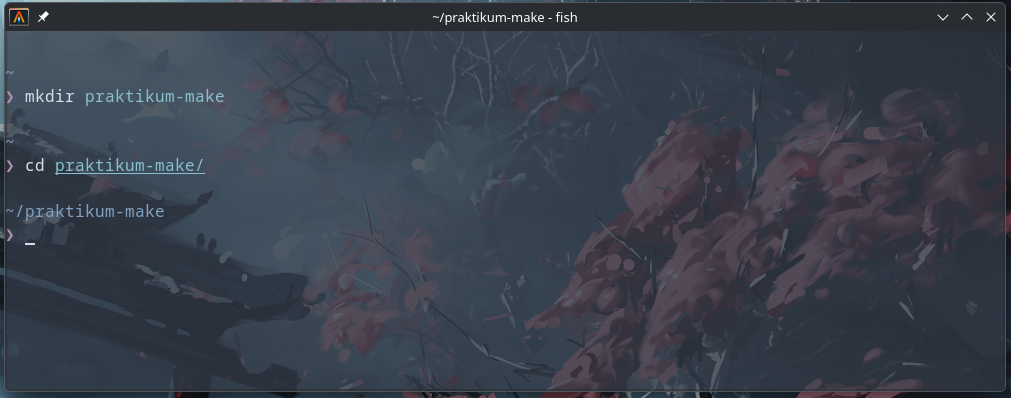
\includegraphics[width=0.75\textwidth]{Figure/06/direktori-make.png}
    \caption{Direktori Kerja Praktikum Modul 6}
    \label{fig:m06-direktori}
\end{figure}
    \item Pastikan instrumen penunjang \texttt{make} terdeteksi di dalam sistem.
    \begin{lstlisting}[language=bash, caption={Mengecek versi Make}]
make --version
    \end{lstlisting}
    \begin{figure}[H]
    \centering
    % TODO: ganti dengan screenshot hasil praktikum
    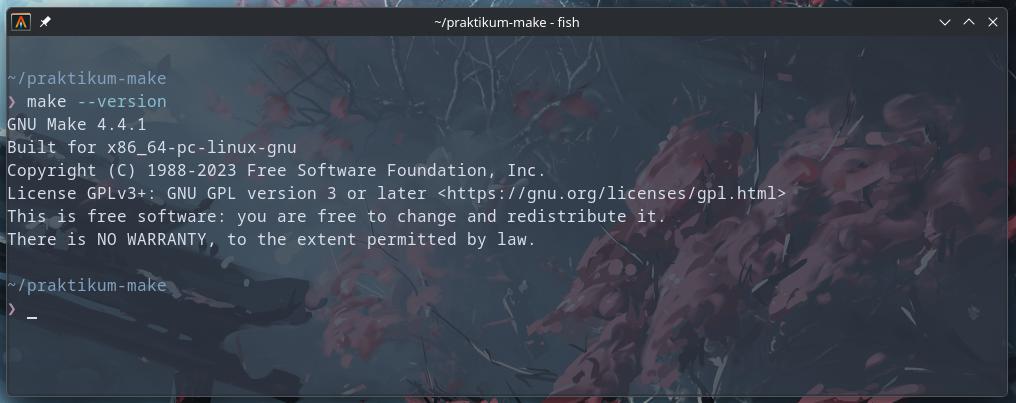
\includegraphics[width=0.75\textwidth]{Figure/06/make-version.png}
    \caption{Validasi Instalasi Make}
    \label{fig:m06-make-version}
\end{figure}

    Jika terminal menampilkan versi rilis (seperti \textit{GNU Make 4.4.1} dsb), Anda siap untuk mendaki ke tahap berikutnya.
\end{enumerate}

\subsection{Sesi 1: Penulisan Makefile Mendasar}
\label{sec:m06-sesi-1}
Di sesi ini, Anda akan memandu kompilasi sebuah kode program C tunggal menggunakan instruksi yang diletakkan dalam berkas \texttt{Makefile}.

\begin{enumerate}
    \item Gunakan editor teks \texttt{nano} untuk menulis berkas program C sederhana. Ketik instruksi ini di terminal:
    \begin{lstlisting}[language=bash, caption={Membuka nano untuk berkas hello.c}]
nano hello.c
    \end{lstlisting}
    Lalu ketik baris berikut ini:
    \begin{lstlisting}[language=c, caption={Isi file hello.c}]
#include <stdio.h>
int main() {
    printf("Ajaib! Program ini dikompilasi oleh Make!\n");
    return 0;
}
    \end{lstlisting}
    \textit{Untuk menyimpan: Tekan dan tahan tombol \textbf{Ctrl}, lalu tekan \textbf{O} (huruf O). Setelah pesan "File Name to Write" di bawah muncul, pencet \textbf{Enter}.}\\
    \textit{Untuk keluar: Tekan \textbf{Ctrl+X}.}

    \begin{figure}[H]
    \centering
    % TODO: ganti dengan screenshot hasil praktikum
    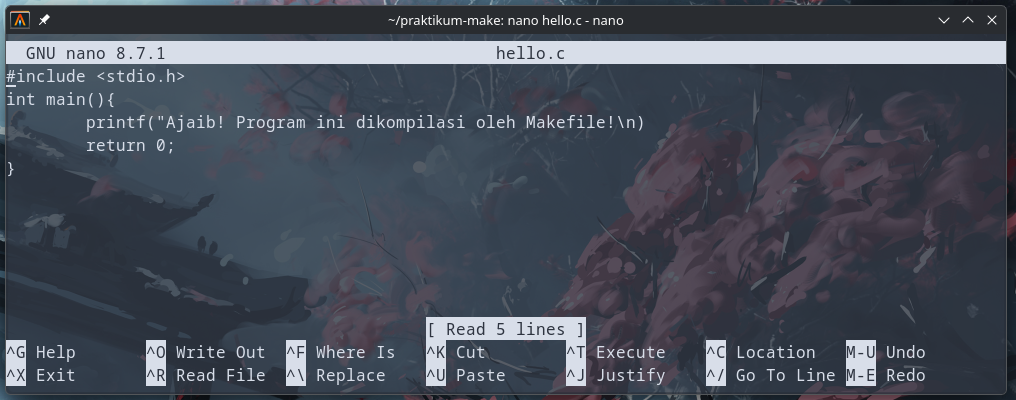
\includegraphics[width=0.75\textwidth]{Figure/06/hello-c.png}
    \caption{Membuat File hello.c dengan Nano}
    \label{fig:m06-hello-c}
\end{figure}

    \item Sekarang, buat instrumen pusat kita, yaitu berkas \texttt{Makefile}. Ingat, huruf 'M' harus dikapitalisasi. Jalankan:
    \begin{lstlisting}[language=bash, caption={Ketik ini di terminal}]
nano Makefile
    \end{lstlisting}

    \item Salin baris berikut. \textbf{SANGAT PENTING:} Di baris ke-2 persis sebelum kursor menyentuh huruf g pada kata `gcc`, Anda TIDAK BOLEH memencet tombol SPASI untuk menjorokkan teks, Anda HARUS MEMENCET TOMBOL \textbf{TAB} (biasanya berada di atas tombol \textit{Caps Lock}). Make sangat ketat terkait aturan penulisan spasi!
    
    \begin{lstlisting}[language=make, caption={Makefile dasar}]
program-halo: hello.c
	gcc hello.c -o program-halo
    \end{lstlisting}
    \textit{Simpan file ini (Ctrl+O, Enter) dan kelur dari nano (Ctrl+X).}

    \begin{figure}[H]
        \centering
        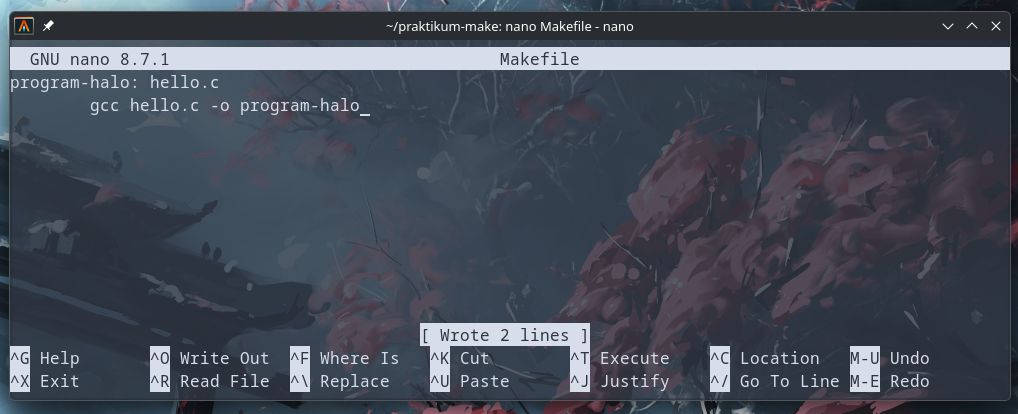
\includegraphics[width=0.75\textwidth]{Figure/06/make.png}
        \caption{Isi Makefile untuk Sesi 1}
        \label{fig:m06-makefile-sesi1}
    \end{figure}


    \item Untuk menginstruksikan \textit{Make} menjalankan target, Anda hanya cukup memanggil \verb|make| tanpa atribut di konsol. 
    \begin{lstlisting}[language=bash, caption={Eksekusi Makefile}]
make
    \end{lstlisting}

    \begin{figure}[H]
        \centering
        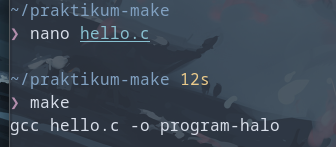
\includegraphics[width=0.75\textwidth]{Figure/06/make-compile.png}
        \caption{Hasil compile dengan Make}
        \label{fig:m06-make-compile}
    \end{figure}

    Perhatikan bahwa \textit{Make} secara otomatis memantulkan perintah `\texttt{gcc hello.c -o program-halo}` ke konsol dan program tersebut telah selesai dikompilasi! Anda dapat membuktikannya dan langsung menjalankannya lewat instruksi:
    \begin{lstlisting}[language=bash, caption={Menjalankan target}]
./program-halo
    \end{lstlisting}

    \begin{figure}[H]
        \centering
        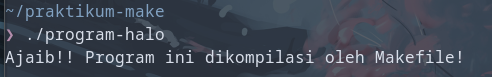
\includegraphics[width=0.75\textwidth]{Figure/06/make-execute.png}
        \caption{Hasil Eksekusi Target program-halo}
        \label{fig:m06-make-execute}
    \end{figure}

    \item Coba jalankan \verb|make| sekali lagi.
    \begin{lstlisting}[language=bash, caption={Jalankan instruksi ini lagi}]
make
    \end{lstlisting}
    Anda akan mendapatkan pesan seperti \textbf{"make: 'program-halo' is up to date"}. Alasan ini adalah inti utama Makefile: Ia mengecek bahwa \texttt{hello.c} (syarat) tidak mengalami perubahan (misalnya kita belum mengeditnya) sejak terakhir kali \texttt{program-halo} (target) dicetak. Karena isinya stabil, \textit{Make} enggan membuang-buang daya waktu dan komputasi!
\end{enumerate}

\begin{figure}[H]
    \centering
    % TODO: ganti dengan screenshot hasil praktikum
    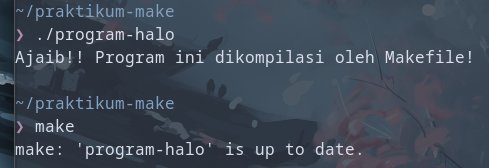
\includegraphics[width=0.75\textwidth]{Figure/06/make-compile-2.png}
    \caption{Hasil Eksekusi dan validasi up-to-date Make}
    \label{fig:m06-make-compile-2}
\end{figure}

\subsection{Sesi 2: Target Kompleks dan Pengunaan Variabel Otomatis}
\label{sec:m06-sesi-2}
Di sesi lanjutan ini, kita akan mereplikasi gaya perakitan berkas asli program-program profesional. Makefile Anda akan merangkum bermacam berkas, membungkus perintah kompilasi ke dalam Variabel Makro, dan mendefinisikan sebuah target baru \texttt{clean} guna membuang sampah file hasil.

\begin{enumerate}
    \item Mari kita buat dua berkas C, satu perpustakaan (`.h`), satu turunan (`.c`), dan satu fungsi gerbang pusar (`.c`).

    \textbf{Bagian 1: Matematika.h}\\
    Jalankan: \texttt{nano matematika.h}
    \begin{lstlisting}[language=c, caption={Isi matematika.h}]
int kali(int x, int y);
    \end{lstlisting}
    \textit{Simpan dan Keluar. (Ctrl+O, Enter $\rightarrow$ Ctrl+X)}

    \begin{figure}[H]
        \centering
        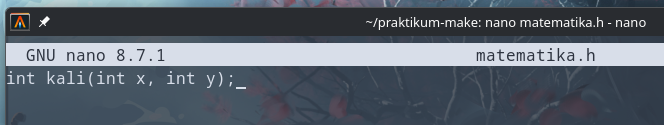
\includegraphics[width=0.75\textwidth]{Figure/06/matematika-h.png}
        \caption{Membuat File matematika.h dengan Nano}
        \label{fig:m06-matematika-h}
    \end{figure}

    \textbf{Bagian 2: Matematika.c}\\
    Jalankan: \texttt{nano matematika.c}
    \begin{lstlisting}[language=c, caption={Isi matematika.c}]
#include "matematika.h"
int kali(int x, int y){
    return x * y;
}
    \end{lstlisting}
    \textit{Simpan dan Keluar. (Ctrl+O, Enter $\rightarrow$ Ctrl+X)}

    \begin{figure}[H]
        \centering
        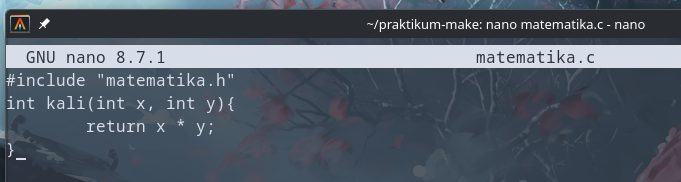
\includegraphics[width=0.75\textwidth]{Figure/06/matematika-c.png}
        \caption{Membuat File matematika.c dengan Nano}
        \label{fig:m06-matematika-c}
    \end{figure}

    \textbf{Bagian 3: Main.c}\\
    Jalankan: \texttt{nano main.c}
    \begin{lstlisting}[language=c, caption={Isi main.c}]
#include <stdio.h>
#include "matematika.h"

int main() {
    printf("Hasil dari 6 dikali 7 adalah: %d\n", kali(6, 7));
    return 0;
}
    \end{lstlisting}
    \textit{Simpan dan Keluar. (Ctrl+O, Enter $\rightarrow$ Ctrl+X)}

    \begin{figure}[H]
        \centering
        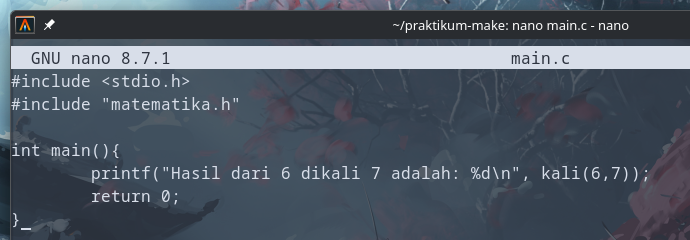
\includegraphics[width=0.75\textwidth]{Figure/06/main-c.png}
        \caption{Membuat File main.c dengan Nano}
        \label{fig:m06-main-c}
    \end{figure}

    \item Sekarang, hapus/timpa isi `Makefile` lama kita sebelumnya dan gunakan skrip utuh canggih berikut.\\
    Jalankan: \texttt{nano Makefile}, kemudian copot/hapus isinya lalu ganti menjadi ini.\\
    \textbf{Pengingat Jarak TAB:} Pastikan untuk setiap lajur baru \textit{Recipe/Perintah terminal} di bawah tulisan berawalan tab, yakni tepatnya berada pada awal baris ke-6 dan ke-9 di bawah ini mengandalkan tombol \lstinline{<TAB>}.

    \begin{lstlisting}[language=make, caption={Makefile Lanjut dengan Macro dan Target}]
CC = gcc
CFLAGS = -Wall

# "$^" bermagnitudo semua prerequisites, "$@" adalah Target yaitu 'aplikasi'
aplikasi: main.c matematika.c
	$(CC) $(CFLAGS) $^ -o $@

# Perintah clean akan merestorasi folder kerja menjadi rapi
clean:
	rm -f aplikasi *.o
    \end{lstlisting}
    \textit{Simpan dan Keluar. (Ctrl+O, Enter $\rightarrow$ Ctrl+X)}

    \begin{figure}[H]
        \centering
        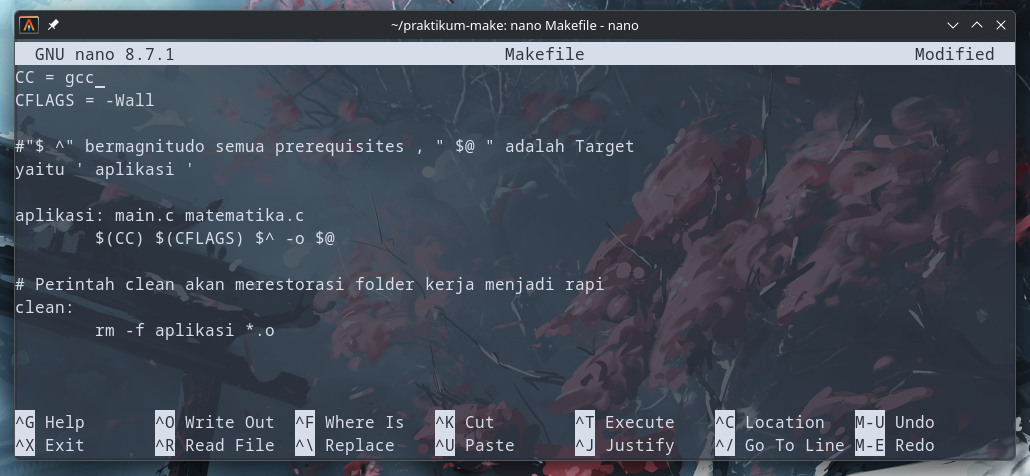
\includegraphics[width=0.75\textwidth]{Figure/06/new-makefile.png}
        \caption{Isi Makefile untuk Sesi 2}
        \label{fig:m06-new-makefile}
    \end{figure}
        

    \item Jalankan proses \textit{Make} yang sekarang akan mendeteksi prasyarat `\texttt{aplikasi}`.
    \begin{lstlisting}[language=bash, caption={Menjalankan multi-file Make}]
make
./aplikasi
    \end{lstlisting}
    Anda akan melihat bahwa Make secara otomatis mengompilasi `main.c` dan `matematika.c` menjadi `aplikasi`, lalu menjalankannya untuk menampilkan hasil perkalian 6 dan 7.
    \begin{figure}[H]
        \centering
        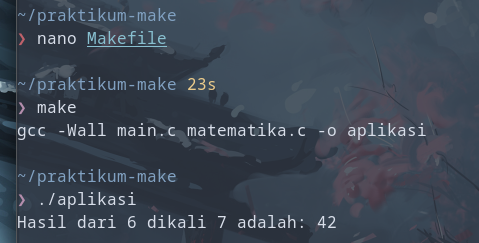
\includegraphics[width=0.75\textwidth]{Figure/06/make-compile-3.png}
        \caption{Hasil Eksekusi Target aplikasi}
        \label{fig:m06-make-compile-3}
    \end{figure}

    \item Terakhir, panggil perintah target buatan Anda untuk mengkandaskan/membersihkan file executable sisa sehingga ruang kerja kembali murni hanya berisi \textit{source code} C saja.
    \begin{lstlisting}[language=bash, caption={Merobohkan file hasil eksekusi}]
make clean
ls
    \end{lstlisting}
    Lihat bagaimana \texttt{ls} kini tidak lagi memampangkan target \texttt{aplikasi} berwarna hijau; Ia telah ludes dan aman dari sisa jejak!
\end{enumerate}

\begin{figure}[H]
    \centering
    \begin{subfigure}[b]{0.45\textwidth}
        \centering
        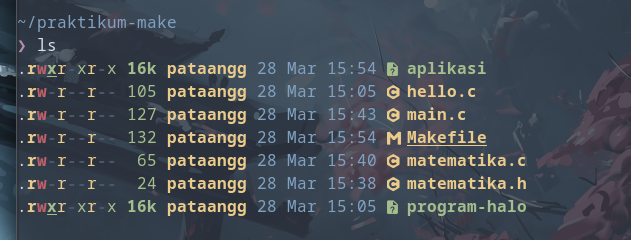
\includegraphics[width=\textwidth]{Figure/06/before-make-clean.png}
        \caption{Sebelum menjalankan \texttt{make clean}}
        \label{fig:m06-before-clean}
    \end{subfigure}
    \hfill
    \begin{subfigure}[b]{0.45\textwidth}
        \centering
        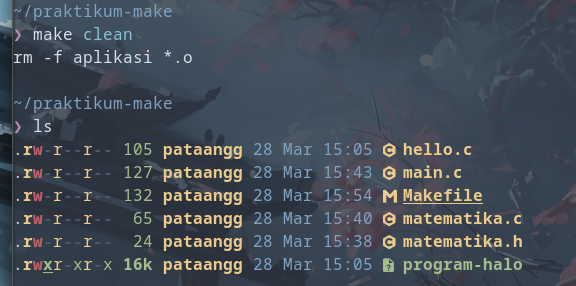
\includegraphics[width=\textwidth]{Figure/06/after-make-clean.png}
        \caption{Setelah menjalankan \texttt{make clean}}
        \label{fig:m06-after-clean}
    \end{subfigure}
    \caption{Perbandingan Direktori Sebelum dan Sesudah Target \texttt{clean} di Makefile}
    \label{fig:m06-make-clean-comparison}
\end{figure}


% --- Tugas mandiri ---
\newpage
\section{Hands-On}
\label{sec:m06-hands-on}

Pada sesi Hands-On ini, Anda akan diminta untuk menggabungkan pengetahuan dari \textbf{Modul 5 (Sistem Build dengan GCC) dan Modul 6 (Otomatisasi dengan Makefile)}. Anda akan membangun sebuah program kalkulator modular sederhana. Buktikan setiap langkah yang Anda lakukan dengan \textit{screenshot} terminal.

\subsection{Tugas 1: Persiapan File Kode Sumber (C)}
\begin{enumerate}
    \item Buatlah sebuah direktori baru bernama \texttt{tugas-kalkulator} dan masuk ke dalamnya.
    \item Buatlah tiga buah file C menggunakan \texttt{nano}:
    \begin{itemize}
        \item \textbf{\texttt{kalkulator.h}} : Berisi deklarasi dua fungsi: \texttt{tambah(int a, int b)} dan \texttt{kurang(int a, int b)}.
        \item \textbf{\texttt{kalkulator.c}} : Berisi implementasi/isi dari fungsi \texttt{tambah} dan \texttt{kurang} tersebut.
        \item \textbf{\texttt{utama.c}} : Berisi fungsi \texttt{main()} yang memanggil fungsi \texttt{tambah(10, 5)} dan \texttt{kurang(10, 5)} lalu mencetak hasilnya ke layar menggunakan \texttt{printf}. Jangan lupa melakukan \texttt{\#include "kalkulator.h"}.
    \end{itemize}
    \item \textbf{Bukti:} Sertakan \textbf{screenshot} kode sumber dari ketiga file tersebut menggunakan perintah \texttt{cat nama\_file}.
\end{enumerate}

\subsection{Tugas 2: Kompilasi Manual dengan GCC (Review Modul 5)}
\begin{enumerate}
    \item Lakukan tahapan kompilasi secara merinci untuk file \texttt{utama.c} dan \texttt{kalkulator.c} hingga menjadi file objek (\texttt{.o}) menggunakan flag \texttt{-c}.
    \item Gabungkan (Link) kedua file objek tersebut (\texttt{utama.o} dan \texttt{kalkulator.o}) menjadi sebuah \textit{executable} utuh bernama \texttt{kalkulator-manual}.
    \item Jalankan \texttt{./kalkulator-manual} untuk memastikan program berjalan dengan benar.
    \item \textbf{Bukti:} Sertakan \textbf{screenshot} perintah-perintah kompilasi GCC tersebut beserta hasil eksekusi programnya.
\end{enumerate}

\subsection{Tugas 3: Mengotomatisasi dengan Makefile (Review Modul 6)}
\begin{enumerate}
    \item Hapus file objek (\texttt{.o}) dan aplikasi *executable* (\texttt{kalkulator-manual}) yang telah Anda buat pada Tugas 2 secara manual (menggunakan perintah \texttt{rm}).
    \item Buatlah sebuah berkas \texttt{Makefile} untuk mengotomatisasi proses pada Tugas 2. 
    \item Pastikan \texttt{Makefile} tersebut memiliki:
    \begin{itemize}
        \item Variabel \texttt{CC} untuk \texttt{gcc}.
        \item Variabel \texttt{CFLAGS} yang minimal berisi \texttt{-Wall}.
        \item Target utama bernama \texttt{kalkulator-otomatis} bermagnitudo dependensi/syarat dari kode C yang Anda buat.
        \item Target \texttt{clean} untuk membersihkan folder kerja dari file \texttt{.o} dan program \textit{executable}.
    \end{itemize}
    \item Jalankan perintah \texttt{make}. Tunjukkan bahwa program berhasil dikompilasi secara otomatis.
    \item Jalankan perintah \texttt{make clean}. Tunjukkan melalui perintah \texttt{ls} bahwa folder kerja Anda kembali bersih.
    \item \textbf{Bukti:} Sertakan \textbf{screenshot} isi \texttt{Makefile} Anda (gunakan \texttt{cat Makefile}), \textbf{screenshot} eksekusi \texttt{make} dan hasil jalannya program, serta \textbf{screenshot} eksekusi \texttt{make clean} dengan bukti folder kembali bersih (\texttt{ls}).
\end{enumerate}